\documentclass[a4paper, 12pt]{article}

\usepackage{sourcesanspro}
\usepackage[T1]{fontenc}
\usepackage[utf8]{inputenc}
\usepackage[document]{ragged2e}
\usepackage{hyperref}
\usepackage{fontawesome5}
\usepackage[tracking=true]{microtype}
\usepackage[scaled=0.90]{helvet}
\usepackage[scaled=0.85]{beramono}
\usepackage{tgpagella}
\usepackage{mathpazo}
\usepackage{mathtools}
\usepackage{amsmath}
\usepackage{amssymb}
\usepackage{amsthm}
\usepackage{scalerel}
\usepackage{bm}
\usepackage{bbm}
\usepackage{xcolor}
\usepackage{enumerate}
\usepackage{soul}
\usepackage{tikz}
\usepackage{listings}
\usepackage{lstbayes}
\usepackage{booktabs}
\usepackage{bold-extra}
\usepackage{textpos}
\usepackage{multirow}
\usepackage{longtable}
\usepackage{tabularx}
\usepackage[flushleft]{threeparttable}
\usepackage{varwidth}

\usepackage{xpatch}
\usepackage[plain]{algorithm}
\usepackage{algorithmicx}
\usepackage[noend]{algpseudocode}

\usepackage{graphicx}
\usepackage{fancybox}


\usepackage[skins,theorems]{tcolorbox}
\tcbset{highlight math style={enhanced,colframe=red,colback=white,arc=0pt,boxrule=1pt}}

%%%%%%%%%%%%%%%%%%%%%%%%%%%%%%%%%%%%%%%%%%%%%%%%%%
% Bibliography settings
%%%%%%%%%%%%%%%%%%%%%%%%%%%%%%%%%%%%%%%%%%%%%%%%%%
\usepackage[backend=biber, style=apa, autocite=inline, doi=false, url=false]{biblatex}
\DeclareLanguageMapping{english}{english-apa}
\setcounter{biburlnumpenalty}{85}  % for urls that are too long
\addbibresource{bibliography.bib}
\setbeamertemplate{bibliography item}{}% Remove reference icon.
\setbeamercolor{bibliography entry author}{fg=bonnblue}
\setbeamercolor{bibliography entry note}{fg=bonnblue}
\renewcommand*{\bibfont}{\footnotesize}
\AtEveryBibitem{%
  \clearfield{volume}%
  \clearfield{number}%
  \clearfield{pages}%
}


%%%%%%%%%%%%%%%%%%%%%%%%%%%%%%%%%%%%%%%%%%%%%%%%%%
% Algorithm
%%%%%%%%%%%%%%%%%%%%%%%%%%%%%%%%%%%%%%%%%%%%%%%%%%
\makeatletter
\xpatchcmd{\algorithmic}{\itemsep\z@}{\itemsep=1ex plus1pt}{}{}
\makeatother



%%%%%%%%%%%%%%%%%%%%%%%%%%%%%%%%%%%%%%%%%%%%%%%%%%
% Math definitions
%%%%%%%%%%%%%%%%%%%%%%%%%%%%%%%%%%%%%%%%%%%%%%%%%%
\newcommand\indicator[1]{\scaleobj{1.4}{\mathbbm{1}} \! \left\{#1\right\}}
\newcommand\expectation[1]{\mathbb{E}\left[#1\right]}

\DeclareMathOperator*{\argmax}{argmax}


%%%%%%%%%%%%%%%%%%%%%%%%%%%%%%%%%%%%%%%%%%%%%%%%%%
% Colors
%%%%%%%%%%%%%%%%%%%%%%%%%%%%%%%%%%%%%%%%%%%%%%%%%%
\definecolor{bonnblue}{RGB}{4, 83, 156}  % hex: #04539C
\definecolor{bonngrey}{RGB}{148, 147, 132}  % hex: #8A9384
\definecolor{bonnyellow}{RGB}{251, 187, 6}  % hex: #FBBB06
\definecolor{red}{RGB}{65, 16, 16}  % hex: #411010

%%%%%%%%%%%%%%%%%%%%%%%%%%%%%%%%%%%%%%%%%%%%%%%%%%
% Auxiliary files
%%%%%%%%%%%%%%%%%%%%%%%%%%%%%%%%%%%%%%%%%%%%%%%%%%
\newcommand{\email}[1]{\def\@email{\texttt{\MakeLowercase{\textls[10]{#1}}}}}

\setbeamerfont{title}{series=\bfseries} % family=\sourcesanspro
\setbeamerfont{subtitle}{series=\scshape, size*={8}{15}} % family=\sourcesanspro
\setbeamercolor{subtitle}{fg=black}
\setbeamerfont{author}{family=\scshape}

\setbeamercolor{title}{fg=black}
\setbeamercolor{author}{fg=bonnblue}
\setbeamercolor{institute}{fg=bonngrey}
\setbeamercolor{email}{fg=bonnyellow}

\defbeamertemplate*{title page}{customized}[1][]
{
    \usebeamerfont{title}\usebeamercolor[fg]{title}\textls[100]{\MakeUppercase{\textbf{\inserttitle}}}\par
    \usebeamerfont{subtitle}\usebeamercolor[fg]{subtitle}\textls[100]{\textsc{\insertsubtitle}}\par\par
    \vfill
    \usebeamerfont{author}\usebeamercolor[fg]{author}\textls[100]{\textsc{\insertauthor}}\par
    \usebeamerfont{institute}{\usebeamercolor[fg]{institute}\textls[100]{\textsc{\insertinstitute}}}\par
    \bigskip
    {\usebeamercolor[fg]{email}\@email}\par
    \usebeamerfont{date}\insertdate\par
    \usebeamercolor[fg]{titlegraphic}\inserttitlegraphic
}



%%%%%%%%%%%%%%%%%%%%%%%%%%%%%%%%%%%%%%%%%%%%%%%%%%
% Auxiliary commands
%%%%%%%%%%%%%%%%%%%%%%%%%%%%%%%%%%%%%%%%%%%%%%%%%%
% \graphicspath{files/} % graphics path
\newcommand{\labelitem}{\tikz\draw[black,fill=bonnblue] (0,0) circle (.35ex); \,\,}

\newcommand{\blue}[1]{\textcolor{bonnblue}{#1}}
\newcommand{\yellow}[1]{\textcolor{bonnyellow}{#1}}
\newcommand{\grey}[1]{\textcolor{bonngrey}{#1}}
\newcommand{\red}[1]{\textcolor{red}{#1}}


%%%%%%%%%%%%%%%%%%%%%%%%%%%%%%%%%%%%%%%%%%%%%%%%%%
% Beamer settings
%%%%%%%%%%%%%%%%%%%%%%%%%%%%%%%%%%%%%%%%%%%%%%%%%%
\setbeamercolor{itemize item}{fg=black}
\setbeamercolor{itemize subitem}{fg=black}
\setbeamercolor{itemize subsubitem}{fg=black}
\setbeamercolor{section head}{fg=cardinal} % currently unused.
\setbeamercolor{footline}{fg=bonnblue}
\setbeamercolor{section in toc}{fg=black}

\setbeamertemplate{itemize item}[circle]
\setbeamertemplate{itemize subitem}{{\textendash}}
\setbeamertemplate{itemize subsubitem}[triangle]
\setbeamertemplate{section in toc}{{\inserttocsectionnumber.}~\inserttocsection}

\setbeamerfont{section in toc}{series=\scshape, size=\Large}
\setbeamerfont{frametitle}{series=\scshape} % \itshape
\setbeamercolor{frametitle}{fg=bonnblue}

\setbeamertemplate{frametitle}
{
    \vspace*{0.4cm}
    \insertframetitle \\ \footnotesize \textcolor{bonngrey}{\insertframesubtitle}
}

\AtBeginSection[]{
  \setbeamertemplate{footline}[frame number]{}
  \setbeamertemplate{navigation symbols}{}
  \setbeamertemplate{footline}{}
  \begin{frame}
  \vfill
  \centering
  \begin{beamercolorbox}[sep=8pt,center]{title}
    {\usebeamerfont{title}\usebeamercolor[fg]{title}{\textsc{\insertsectionhead}}}\par%
  \end{beamercolorbox}
  \vfill
  \end{frame}
  \addtobeamertemplate{navigation symbols}{}{%
      \usebeamerfont{footline}%
      \usebeamercolor[fg]{author}%
      \hspace{1em}%
      \raisebox{1em}[0pt][0pt]{%
      \small \insertframenumber/\inserttotalframenumber \kern 0.25em
      }
  }
}

\AtBeginSubsection[]{
  \setbeamertemplate{footline}[frame number]{}
  \setbeamertemplate{navigation symbols}{}
  \setbeamertemplate{footline}{}
  \begin{frame}
  \vfill
  \centering
  \begin{beamercolorbox}[sep=8pt,center]{title}
      {\usebeamerfont{title}\usebeamercolor[fg]{title}{\textsc{{\normalsize
      \grey{\insertsectionhead}}\\[1em] \insertsubsectionhead}}}\par%
  \end{beamercolorbox}
  \vfill
  \end{frame}
  \addtobeamertemplate{navigation symbols}{}{%
      \usebeamerfont{footline}%
      \usebeamercolor[fg]{author}%
      \hspace{1em}%
      \raisebox{1em}[0pt][0pt]{%
      \small \insertframenumber/\inserttotalframenumber \kern 0.25em
      }
  }
}



% Title page
\title{\textbf{Final Project}\\
    \large \textit{Point-of-Impact Models with Functional Predictors}\\[1em]
    \Large Topics in Econometrics and Statistics, Summer, 2021
}
\date{}
\author{Tim Mensinger%
  \thanks{\href{mailto:tmensinger@uni-bonn.de}{tmensinger[at]uni-bonn.de}}}
\affil{University of Bonn}


\begin{document}

\onehalfspacing


\maketitle
\begin{abstract}
    In this essay I introduce the core insights presented in \cite{Kneip2020}. I extend
    their work by following up on a remark in the paper, allowing for a less restrictive
    assumption on the functional regressors. I add functionality to the existing
    \textsf{R}-package and compare results using a Monte-Carlo study. All materials
    needed to reproduce this project can be found online\footnote{Online repository:
    \url{https://github.com/timmens/topics-metrics-2021}}. This essay is \emph{not}
    designed to be read fully independent from the original paper.
\end{abstract}
\thispagestyle{empty}

\newpage

\section{Introduction}


\subsection{Motivation}

\begin{frame}{Paper}{Liebl et al. (2020)}
\begin{figure}[ht]
    \centering
    \vspace{-0.8cm}
    \shadowbox{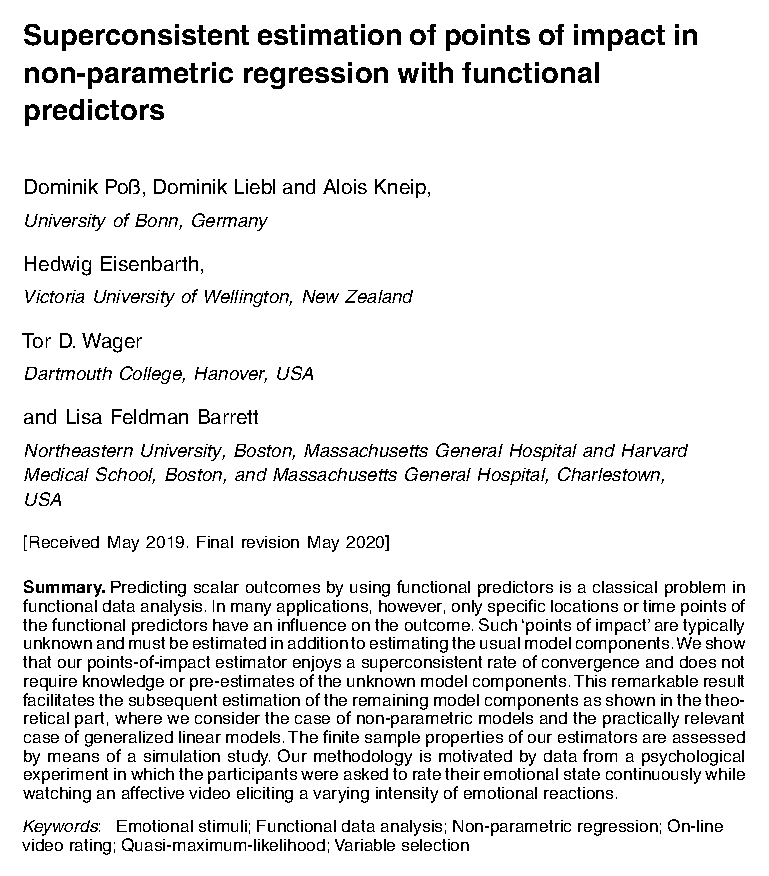
\includegraphics[width=0.45\textwidth]{files/paper-titlepage.pdf}}
\end{figure}
\end{frame}

\begin{frame}{The Setting}{Liebl et al. (2020)}
\begin{figure}[ht]
    \centering
    \vspace{-1cm}
    
\includegraphics[width=0.55\textwidth]{files/drawing.pdf}
    \fbox{
\includegraphics[width=0.35\textwidth]{files/video-snapshot.pdf}}\\[0.5em]
    \hspace{7.7cm} \footnotesize Figure 1: Snapshot of YouTube video
\end{figure}
\end{frame}

\begin{frame}{The Setting}
    \vspace{-1cm}
    \hspace{0.5cm}
    \begin{centering}
     \begin{tikzpicture}

         % time line
         \draw[line width=0.25mm, ->] (-3.75,0) -- (3.5,0) node [below] {};
         \draw (-3.25, -0.1) -- (-3.25, 0.1) node [below] {\shortstack{\\ \footnotesize Video Start}};
         \draw (2.5, -0.1) -- (2.5, 0.1) node [below] {\shortstack{\\ \footnotesize Video End}};

         % horizontal scale
         \draw[line width=0.25mm] (7, -3) -- (7, 3) node [above] {Sentiment};
         \foreach \x in {-3,-2,...,3}
            \draw (6.8, \x) -- (7.2, \x);

         \node[align=right] at (7.5, 0) {$0$};
         \draw[color=bonnblue, line width=0.3mm] (6.8, 1) -- (7.2, 1);

         % time-point
         \draw[line width=0.3mm, color=bonnblue] (-1, 0.1) -- (-1, -0.1);
         \node[] at (-1, -0.75) {\textcolor{bonnblue}{$\bm{t}$}};
         \draw[color=bonnblue, line width=0.3mm, ->] (-1, 0.25) .. controls (1, 1) and
             (3, 3) .. (5.5, 1) node [right] {\textcolor{bonnblue}{$\bm{X_i(t)}$}};

         \pause
         
         % outcome
         \draw[color=bonngrey, line width=0.3mm, ->] (2.5, -0.5) .. controls (2, -2) and (1.25, -2.2) .. (0, -2.5) node [left] {\textcolor{bonngrey}{$\bm{Y_i} \in \{0, 1\}$}};
         
     \end{tikzpicture}
 \end{centering}
\end{frame}


\newcommand{\brownianmotion}[5]{% points, advance, rand factor, options, end label
\draw[#4] (0,0)
\foreach \x in {1,...,#1}
{   -- ++(#2,rand*#3)
}
node[right] {#5};
}

\begin{frame}{The Data}{Regressors}
\pgfmathsetseed{1341}
\begin{centering}
\begin{tikzpicture}
    \draw[line width=0.25mm, ->] (0, -2) -- (0, 3);
    \draw[line width=0.25mm, ->] (-1, 0) -- (11, 0) node [below] {$t$};
    \brownianmotion{180}{0.05}{0.25}{color=bonngrey, line width=0.2mm}{$X_3(t)$}
    \brownianmotion{180}{0.05}{0.25}{color=bonnyellow, line width=0.2mm}{$X_2(t)$}
    \brownianmotion{180}{0.05}{0.25}{color=bonnblue, line width=0.2mm}{$X_1(t)$}
\end{tikzpicture}
\end{centering}
\end{frame}


\begin{frame}{The Problem}
\pgfmathsetseed{1341}
\vspace{-1cm}
\begin{tikzpicture}[scale=0.8]

    \draw[line width=0.25mm, ->] (0, -2) -- (0, 3);
    \draw[line width=0.25mm, ->] (-1, 0) -- (11, 0) node [below] {$t$};
    \brownianmotion{180}{0.05}{0.25}{color=bonngrey, line width=0.2mm}{$X_3(t)$}
    \brownianmotion{180}{0.05}{0.25}{color=bonnyellow, line width=0.2mm}{$X_2(t)$}
    \brownianmotion{180}{0.05}{0.25}{color=bonnblue, line width=0.2mm}{$X_1(t)$}

    \node[] at (12, 4) {$Y_1 \simeq g\big(X_1(\tau_1), X_1(\tau_2)\big)$};

    \draw[line width=0.2mm, dashed] (2, 4) -- (2, -3) node [right] {$\tau_1$};
    \draw[line width=0.2mm, dashed] (5, 4) -- (5, -3) node [right] {$\tau_2$};

    \node[circle, draw=black, minimum size=1mm, scale=0.9] (c1) at (2, 1.9) {};
    \draw[line width=0.2mm, ->] (c1) .. controls (3, 6) and (10, 6) .. (11.5, 4.5);

    \node[circle, draw=black, minimum size=1mm, scale=0.9] (c2) at (5, 2.6) {};
    \draw[line width=0.2mm, ->] (c2) .. controls (10, 2) and (12.5, 2.5) .. (13, 3.6);

\end{tikzpicture}
\end{frame}


\subsection{The Model}

\begin{frame}{The Model}

    \vspace{-1cm}
    \begin{align*}
        \tcbhighmath[fuzzy halo=1mm with bonnblue,arc=2pt, boxrule=0pt,frame
        hidden]{
            Y_i = g\left(X_i(\tau_1), \dots, X_i(\tau_S) \right) +  \epsilon_i
        }
    \end{align*}

    \vspace{0.5cm}
    \begin{table}[]
    \renewcommand{\arraystretch}{1.5}
        \begin{tabular}{ll}
          \labelitem $X_i = \{ X_i(t) : t \in [0, 1]\}$ & square integrable process\\
          \labelitem $\mathbb{E}\left[\epsilon_i \mid X_i(t) \right] = 0$ &  exogeneity\\
          \labelitem $g : \mathbb{R}^S \to \mathbb{R}$ & \emph{unknown} link function \\
          \labelitem $\tau_1, \dots, \tau_S \in [0, 1]$ &  \emph{unknown} points of impact
        \end{tabular}
    \end{table}

\end{frame}


\begin{frame}{Approach}

    \begin{table}[]
    \renewcommand{\arraystretch}{1.5}
        \begin{tabular}{ll}

        \textcolor{bonnblue}{$1$. stage} & Estimate $S$ and $\tau_1, \dots, \tau_S$\\
        \textcolor{bonnblue}{$2$. stage} & Estimate link function $g$

        \end{tabular}
    \end{table}

    \vspace{1cm}
    \emph{Focus here:} 1. stage

\end{frame}

\section{Review}
\label{section:review}

In this section I present the general setting of \cite{Kneip2020}, albeit restricted to
the definitions, assumptions and theorems that are needed to understand the extension in
section \ref{section:extension}. We assume there is an independent and identically
distributed sample of data $(X_i, y_i)$ for $i=1,\dots,n$ individuals. The functional
regressors $X_i = \{ X_i(t) : t \in [a, b] \}$ is assumed to be a square-integrable
process and $y_i$ is a real-valued random variable. The relationship between regressors
and outcome is modeled as

\[
    y_i = g \left( X_i(\tau_1), \dots, X_i(\tau_S) \right) + \epsilon_i \,,
\]

with $\epsilon_i$ representing the error term satisfying $\expectation{\epsilon_i \mid
X_i(t)} = 0$ for all $t \in [a, b]$. The points of impact are denoted by $\tau_1, \dots,
\tau_S$; where the specific locations $\tau_s \in [a, b]$ are assumed to be unknown a
priori, as well as the number of points $S \in \mathbb{N}_0$. In the same way the link
function $g$ is assumed to be unknown as well. The paper considers centred random
functions $X_i$.

Now one may question how it is possible to estimate the locations as well as their
number while allowing the link function $g$ to be flexible. The upcoming repetitions of
the main assumptions and theorems in \cite{Kneip2020} illustrate that restrictions on
$X_i$ through the covariance kernel suffice for the identification and estimation.

Consider first the covariance kernel of the functional regressor. Let $\sigma(t, s) =
\expectation{X_i(t) X_i(s)}$ denote the covariance kernel of $X_i$.


\begin{assumption}
    Given the kernel $\sigma$, there exists open $\Omega \subset [0, 1]^3$ and twice
    continuously differentiable function $\omega : \Omega \to \mathbb{R}$, as well as
    some $\kappa \in (0, 2)$, such that $\forall s, t \in [0, 1]$

    \[
        \sigma(s, t) = \omega(s, t, |s-t|^{\kappa}) \,.
    \]

    Moreover, $0 < \inf \left\{ c(t) : t \in [0, 1] \right\}$, where $c(t) =
    -\frac{\partial}{\partial z} \omega(t, t, z)|_{z = 0} \,.$
\label{assumption:1}
\end{assumption}

Assumption \ref{assumption:1} restricts the degree of smoothness at the diagonal using
the parameter $\kappa$. This in turn implies certain behavior of the sample paths of the
process. Values with $\kappa < 2$ suggest non-smooth trajectories, while processes with
smooth sample paths and twice continuously differentiable kernel will satisfy the
assumption with $\kappa = 2$. That is, in the current form assumption \ref{assumption:1}
implies that the sample paths of the regressors $X_i$ need to be somewhat rough. Many
known processes fulfill assumption \ref{assumption:1}, for example, Brownian Motion
fulfills it with $\kappa = 1$. In section \ref{section:extension} I present an extension
to this assumption with $\kappa > 2$, allowing for a greater number of processes to be
modeled.


The ability to identify and estimate the points-of-impact relies heavily on the
decomposition presented in theorem \ref{theorem:1}.


\begin{theorem}
Let $X_i$ be a Gaussian process and $g : \mathbb{R}^S \to \mathbb{R}$ an arbitrary
function with continuous partial derivatives almost everywhere. For $s=1,\dots,S$ define

\[
    \vartheta_s = \expectation{\frac{\partial}{\partial x_s} g(X_i(\tau_1), \dots,
    X_i(\tau_S))} \,.
\]

If $0 < \left| \vartheta_s \right| < \infty, \forall s=1,\dots,S$, then we may write,
$\forall t \in [a, b]$

\[
    f_{XY}(t) \stackrel{def}{=} \expectation{X_i(t) y_i} = \sum_{s=1}^S \vartheta_s
    \sigma(t, \tau_s) \,.
\]
\label{theorem:1}
\end{theorem}


Let us henceforth call $f_{XY}$ the cross-covariance (between $X_i$ and $y_i$). In light
of assumption \ref{assumption:1} we know that the kernel $\sigma$ is \emph{not}
two-times differentiable at the diagonal. But then $f_{XY}$ will not be two-times
differentiable at the points-of-impact $\tau_1, \dots, \tau_S$. As it turns out, this
will be enough to ensure identification of the points-of-impact. To differentiate
between any point ($t \in [a, b]$) and a point-of-impact ($t = \tau_s$ for some $s$) the
paper proposes the measure

\[
    f_{ZY}(t) \stackrel{def}{=} f_{XY}(t) - \frac{1}{2} \left( f_{XY}(t + \delta) +
    f_{XY}(t - \delta) \right) \,,
\]

with hyper-parameter $\delta > 0$. Under our current set of assumptions the function
$f_{ZY}$ will be large in absolute value for $t$ close to a point-of-impact. This allows
for the estimation of the points-of-impact using extremum points of an estimated version
of $|f_{ZY}|$. But what is $f_{ZY}$ actually measuring? Notice that the second-order
finite difference of $f_{XY}$ is given by

\begin{align*}
    FD(f_{XY}, \delta, 2)(x) &= \left( f(x + \delta) + f(x - \delta) \right) - 2 f(x)\\
                             &= - \frac{1}{2} f_{ZY}(x) \,,
\end{align*}

where $FD(h, \delta, \ell, x)$ denotes the $\ell$-th order finite difference of function
$h$ with step length $\delta$, evaluated at $x$. Since the criterion function is in
absolute value we can see that using $f_{ZY}$ is proportional to second-order finite
difference of $f_{XY}$. This should make sense, as assumption \ref{assumption:1} implied
that $f_{XY}$ should not be two-times differentiable at the points-of-impact. In that
case, the second-order finite difference formula is expected to be larger at the
points-of-impact than at the other time points.


With this new interpreation in mind we may ask whether we can exploite higher-order
finite differences to relax the assumption on the covariance kernel? The answer is
affirmative and the details will be the concern of section \ref{section:extension}.


At last I state the original version of the estimation algorithm as a comparison to the
more general version supplied in the next section. For the estimation stage we suppose
that the functional regressors $X_i$ are observed at $p$ equidistant points $t_1, \dots,
t_p$ with $t_1 = a, t_p = b$. Since the functions $f_{XY}$ and $f_{ZY}$ are simple
functions of expectations, they can be easily estimated by the standard sample
counterpart, which we denote by $\hat{f}_{XY}$ and $\hat{f}_{ZY}$. The orignal algorithm
is listed as algorithm \ref{algorithm:1}.

\begin{tcolorbox}[standard jigsaw, opacityback=0]

\begin{algorithm}[H]
\caption{Original algorithm from \cite{Kneip2020}, adapted for readability.}
\label{algorithm:1}
\begin{algorithmic}[1]
  \State compute $\hat{f}_{XY}(t_j) = \sum_i X_i(t_j) Y_i / n$, for all $j=1,\dots,p$
  \State choose $\delta > 0$ s.t. $\exists \, k_{\delta} \in \mathbb{N}$ with $1 \leq
  k_{\delta} < (p - 1)/2$ and $\delta = k_{\delta} / (p-1)$
  \State define $\mathcal{J}_{\delta} = \{k_{\delta} + 1, \dots, p - k_{\delta}\}$ and
  set $\ell = 1$
  \State compute $\hat{f}_{ZY}(t_j) = \hat{f}_{XY}(t_j) - (\hat{f}_{XY}(t_j + \delta) +
  \hat{f}_{XY}(t_j - \delta)) / 2$, for all $j \in \mathcal{J}_{\delta}$
  \While{$\mathcal{J}_{\delta} \neq \varnothing$}
  \State estimate $\hat{\tau}_{\ell} = \argmax \left\{|\,\hat{f}_{ZY}(t_j)| : \text{for }
      t_j \text{ with } j \in \mathcal{J}_{\delta}\right\}$
    \State update $\mathcal{J}_{\delta} \leftarrow \mathcal{J}_{\delta} \setminus
    [\hat{\tau}_{\ell} - \sqrt{\delta}, \hat{\tau}_{\ell} + \sqrt{\delta}]$
    \State update $\ell \leftarrow \ell + 1$
  \EndWhile
  \State \textbf{return} $\{\hat{\tau}_{\ell}\}$
\end{algorithmic}
\end{algorithm}

\end{tcolorbox}

\section{Extension}
\label{section:extension}

\textcolor{red}{\lipsum}

\section{Monte-Carlo Study}
\label{section:monte_carlo}

In this last section I test the aforementioned extension using a simulation study.

The Monte-Carlo design compares an application of Algorithm \ref{algorithm:2} for $d \in
\{2, 4\}$. To gain a better understanding on the criticality of Assumption
\ref{assumption:1}, and its relaxation, I consider a parameterized functional regressor
which allows me to choose the level of local variation.

\paragraph{Setup.}

The data generating process is setup as follows. For a given smoothness parameter $\nu
\in \{0.5, 1.5, 2.5\}$, the functional regressors $X_i$ are simulated as a mean-zero
Gaussian process with a Matern covariance kernel using length scale parameter $\ell =
0.1$ and smoothness parameter $\nu$ ---a mathematical description of the Matern kernel
and its relation to Assumption \ref{assumption:1} is provided in the next paragraph. The
process is observed for $T=100$ periods on an equidistant grid. I compare how the method
performs for $S \in \{0, 1, 2\}$ points-of-impact. In the case of $S = 1$ the location
is given by $\tau_1 = 49$. And in the case of $S = 2$ we have $(\tau_1, \tau_2) = (24,
49)$. Given the number of points-of-impact $S$, the coefficient vectors are fixed with:
$\beta_0 = (1)$, $\beta_1 = (1, 2)$ and $\beta_2 = (1, 2, -1)$. The outcomes are then
simulated using
\[
    y_i = \beta_{S, 0} + \sum_{r = 1}^S \beta_{S, r} \, X_i(\tau_r) + \epsilon_i \,,
\]
where $\epsilon_i$ is an i.i.d. Gaussian error with $Var(\epsilon_i) = 1/2$. Note that
$\beta_{S, r}$ denotes the $r$-th entry of the $(S+1)$-dimensional coefficient vector,
in the case of $S$ number of points-of-impact. The number of observations is fixed to $n
= 100$. In principle, it would be interesting to see how the results depend on the
sample size; however, for the sake of clarity I refrain from analyzing this dimension.

Figure \ref{figure:process_scale_comparison} illustrates three simulated sample paths of
the functional regressor, for the three different smoothness parameters $\nu$. As is
clearly visible, for small $\nu$ (top row) the process possesses a lot of local
variation, while for larger $\nu$ (bottom row) the process is much smoother with a low
level of variation.


\begin{figure}

\centering
\begin{subfigure}[b]{\textwidth}
\begin{tcolorbox}[standard jigsaw, opacityback=0, top=0pt, left=0pt, right=0pt, bottom=0pt]
    \includegraphics[height=0.2\pdfpageheight,
    width=0.98\textwidth]{../../bld/figures/process_scale0.5}
\end{tcolorbox}
\end{subfigure}

\hfill

\begin{subfigure}[b]{\textwidth}
\centering
\begin{tcolorbox}[standard jigsaw, opacityback=0, top=0pt, left=0pt, right=0pt, bottom=0pt]
    \includegraphics[height=0.2\pdfpageheight,
    width=0.98\textwidth]{../../bld/figures/process_scale1.5}
\end{tcolorbox}
\end{subfigure}

\hfill

\begin{subfigure}[b]{\textwidth}
\centering
\begin{tcolorbox}[standard jigsaw, opacityback=0, top=0pt, left=0pt, right=0pt, bottom=0pt]
    \includegraphics[height=0.2\pdfpageheight,
    width=0.98\textwidth]{../../bld/figures/process_scale2.5}
\end{tcolorbox}
\end{subfigure}

\caption{Simulated trajectories of a Gaussian process with Matern kernel and differing
smoothness parameter; top: $\nu = 0.5$; center: $\nu = 1.5$; bottom: $\nu = 2.5$.}
\label{figure:process_scale_comparison}
\end{figure}


\paragraph{The Kernel.}

For this study I choose kernels from the Matern class. Explicitly, the kernel is defined
by

\[
    \sigma(s, t) = \frac{2^{1 - \nu}}{\Gamma(\nu)} \left(
    \frac{\sqrt{2 \nu} |s - t|}{\ell} \right)^\nu K_{\nu} \left( \frac{\sqrt{2 \nu} |s -
    t|}{\ell} \right) \,,
\]
with length scale parameter $\ell > 0$ and smoothness parameter $\nu > 0$. Note that
$\Gamma$ denotes the usual gamma function, while $K_{\nu}$ is a modified Bessel
function. For a more detailed reference on the components of the Matern kernel, as well
as a reference for the following properties, see \cite{Rasmussen2006}. The above
expression is hard to work with. Luckily, for the special cases $\nu \in \{0.5, 1.5,
2.5\}$ it simplifies dramatically, as is shown in Table \ref{table:matern_kernel}, where
I define $z = |s - t|$.

\smallskip

\begin{remark}
I must note that, for the case of $\kappa < 2$, neither the Matern kernel with $\nu =
1.5$ nor with $\nu = 2.5$ satisfy Assumption \ref{assumption:1}. This is because $\inf
\{ c(t) : t \in [0, 1] \} = 0$ in these cases. That means that the covariance at the
diagonal does not drop off fast enough.  Furthermore, an extension of the assumption to
the case $\kappa < 4$ is not of help either, as the partial derivative $\partial \omega
/ \partial z$ is not defined at $z = 0$ for any $\kappa > 1$. To analyze the extended
method properly one would need to use a kernel satisfying an extended version of
Assumption \ref{assumption:1} with $\kappa \in [2, 4)$. It proved difficult to find a
reasonable kernel for this case. As the sample paths induced by the Matern kernel with
high $\nu$ are fairly standard, the results should, nevertheless, still tell us
something of relevance about the underlying method.
\end{remark}


\begin{table}
    \renewcommand{\arraystretch}{2}
    \centering
    \begin{tabular}{c|c}
        $\nu$ & $\sigma_{\text{Matern}}(z)$ \\ \hline
        $1/2$ & $\exp \left( - z / \ell \right)$\\
        $3/2$ & $\left(1 + \sqrt{3} z / \ell \right)\exp \left( - \sqrt{3}z / \ell \right)$\\
        $5/2$ & $\left(1 + \sqrt{5} z / \ell + 5z^2 / (3\ell^2) \right)\exp \left( -
        \sqrt{5}z / \ell \right)$
    \end{tabular}
    \caption{Simple expressions of the Matern kernel for special cases of the smoothness
    parameter $\nu$; see \cite{Rasmussen2006}. Here $z = |s - t|$.}
    \label{table:matern_kernel}
\end{table}



\paragraph{Monte-Carlo Design.}

I perform 500 Monte-Carlo repetitions over the parameter grid spanned by $d \in \{2, 4\},
S \in \{0, 1, 2\}$ and $\nu \in \{0.5, 1.5, 2.5\}$. The results are visualized using
frequency plots that summarize the estimated points-of-impact over \emph{all}
Monte-Carlo repetitions. A detailed explanation follows in the next paragraph.
Alternatively, one could have computed e.g. the Hausdorff-distance between the true and
estimated points-of-impact in each simulation run, or reported the average number of
estimated points-of-impact. For the sake of brevity I stick to one way of reporting the
results. Furthermore, in this study I focus only on the estimation of the
points-of-impact and not on the subsequent estimation of the coefficient parameters.


\paragraph{Results.}

Before we consider the actual results, let us think about what we may expect. The slope
parameter corresponding to the second point-of-impact is significantly smaller than the
one corresponding to the first point-of-impact. Hence, in the case of $S = 2$ we should
expect that the method finds the first point-of-impact at least as often. We also expect
that the precision of the method decreases in $\nu$, i.e. the smoother the functional
regressor the less precise the estimates. For the case of $S = 0$ we should see no
difference for varying smoothness nor for varying $d$. What we hope to see is that for
the case $d = 4$, i.e. when using the fourth-order finite difference, the performance of
the method increases in the smoother $\nu = 2.5$ case.

Figure \ref{figure:monte_carlo_results_order2} summarizes the results when applying the
standard algorithm ($d = 2$). The top row shows the case of no points-of-impact ($S =
0$), the center row depicts the case of one point-of-impact ($S = 1$) and the bottom row
exhibits the case of two points-of-impact ($S = 2$). The results are consistent with our
expectations. The plot can be understood as follows: In the middle sub-figure we see
that for the $\nu = 0.5$ case the true location ($49$) makes up more than $50\%$ of the
estimated locations. In all cases for $\nu$ and both cases for $d$ we see no difference
in the frequency of false-positives (top row).

Even though Assumption \ref{assumption:1} is not satisfied for $\nu \in \{1.5, 2.5\}$,
the estimated locations form a cluster around the true points. This should tell us that
a mild violation of Assumption \ref{assumption:1} does not ruin the analysis completely
and that an improved criterion function may result in even more precise estimates. The
large variance is also in line with the argumentation of \cite{Kneip2020}, in that the
smooth functional regressors make it harder for the method to distinguish between the
influence of neighboring points.

Figure \ref{figure:monte_carlo_results_order4} depicts the case when employing the
fourth-order finite difference ($d = 4$). The image is similar to the above figure.
However, a main difference is that the precision is lower than in the $d=2$ case.
Especially in the smooth cases the method performs worse, as there are no sharp peaks
and the estimated points are spread over a large area.

The observation from Figure \ref{figure:monte_carlo_results_order4} may be due to
several reasons. First, as stated in the aforementioned remark, the kernel used to
simulate the functional regressors does not satisfy the extended Assumption
\ref{assumption:1}. The method remains to be tested with such a kernel. A
counter-argument would be that in the coarsely discretized case the regressors will
almost certainly look similar to the ones I am using here. Second, the fourth-order
finite difference formula may not be precise enough. One could think about modifying
this measure slightly to get a more precise criterion function.

\begin{figure}

\begin{subfigure}[b]{\textwidth}
\centering
\includegraphics[width=\textwidth]{../../bld/figures/monte_carlo/barplot_2_0}
\end{subfigure}

\begin{subfigure}[b]{\textwidth}
\centering
\includegraphics[width=\textwidth]{../../bld/figures/monte_carlo/barplot_2_1}
\end{subfigure}

\begin{subfigure}[b]{\textwidth}
\centering
\includegraphics[width=\textwidth]{../../bld/figures/monte_carlo/barplot_2_2}
\end{subfigure}

\caption{Results from 500 Monte-Carlo repetitions. Length scales are differentiated
using color; orange: $\nu = 0.5$; green: $\nu = 1.5$; blue: $\nu = 2.5$. In this
Monte-Carlo run Algorithm \ref{algorithm:2} was used with order $d = 2$. True
points-of-impact are depicted by the red vertical line.}
\label{figure:monte_carlo_results_order2}
\end{figure}

\begin{figure}

\begin{subfigure}[b]{\textwidth}
\centering
\includegraphics[width=\textwidth]{../../bld/figures/monte_carlo/barplot_4_0.pdf}
\end{subfigure}

\begin{subfigure}[b]{\textwidth}
\centering
\includegraphics[width=\textwidth]{../../bld/figures/monte_carlo/barplot_4_1.pdf}
\end{subfigure}

\begin{subfigure}[b]{\textwidth}
\centering
\includegraphics[width=\textwidth]{../../bld/figures/monte_carlo/barplot_4_2.pdf}
\end{subfigure}

\caption{Results from 500 Monte-Carlo repetitions. Length scales are differentiated
using color; orange: $\nu = 0.5$; green: $\nu = 1.5$; blue: $\nu = 2.5$. In this
Monte-Carlo run Algorithm \ref{algorithm:2} was used with order $d = 4$. True
points-of-impact are depicted by the red vertical line.}
\label{figure:monte_carlo_results_order4}
\end{figure}


\printbibliography


\end{document}
